\documentclass[11pt,a4paper]{article}

% --- Packages ---
\usepackage[utf8]{inputenc}
\usepackage[margin=1in]{geometry}
\usepackage{amsmath,amssymb,amsfonts}
\usepackage{graphicx}
\usepackage{booktabs}
\usepackage{multirow}
\usepackage{tabularx}
\usepackage[dvipsnames,table]{xcolor}
\usepackage{fancyhdr}
\usepackage{hyperref}
\usepackage{tcolorbox}
\usepackage{enumitem}
\usepackage{caption}
\usepackage{subcaption}
\usepackage{cite}
\usepackage{microtype}
\usepackage{float}

% --- Custom Colors ---
\definecolor{NavyBlue}{RGB}{20, 50, 110}
\definecolor{ForestGreen}{RGB}{20, 130, 60}
\definecolor{Crimson}{RGB}{180, 20, 30}
\definecolor{DarkSlate}{RGB}{30, 41, 59}
\definecolor{LightBlueBox}{RGB}{240, 246, 255}
\definecolor{BorderBlue}{RGB}{59, 130, 246}

% --- Hyperref Setup ---
\hypersetup{
    colorlinks=true,
    linkcolor=NavyBlue,
    citecolor=NavyBlue,
    urlcolor=NavyBlue,
    pdftitle={Everyday Waste Sorting via Manual Image Descriptors and Transfer Learning},
    pdfauthor={Team 41 - Vansh Sharma, Shyam Verma, Swati Ghosh, Anshu, Yash}
}

% --- Header and Footer Styling ---
\pagestyle{fancy}
\fancyhf{}
\fancyhead[L]{\small \textit{Everyday Waste Sorting via Manual Image Descriptors and Transfer Learning}}
\fancyhead[R]{\small \textit{Team 41 --- AML (CSAI)}}
\fancyfoot[C]{\thepage}
\renewcommand{\headrulewidth}{0.4pt}
\renewcommand{\footrulewidth}{0pt}

% --- Callout Box Setup ---
\tcbset{
    boxrule=1pt,
    arc=3pt,
    left=10pt,
    right=10pt,
    top=8pt,
    bottom=8pt,
    colback=LightBlueBox,
    colframe=BorderBlue,
    fonttitle=\bfseries\color{white},
    coltitle=white,
    colbacktitle=BorderBlue
}

\begin{document}

% =========================================================================
% PAGE 1: TITLE PAGE
% =========================================================================
\begin{titlepage}
    \centering
    \vspace*{0.8cm}
    
    {\scshape\Large Department of Computer Science and Artificial Intelligence \par}
    \vspace{0.2cm}
    {\scshape\large School of Technology, Rishihood University \par}
    \vspace{0.2cm}
    {\scshape\normalsize Sonipat, Haryana, India \par}
    
    \vspace{2.2cm}
    
    {\huge\bfseries Everyday Waste Sorting via \\[0.3cm]
    Manual Image Descriptors and \\[0.3cm]
    Transfer Learning \par}
    
    \vspace{0.8cm}
    {\large\textit{Comprehensive Evaluation on the TrashNet Dataset: Investigating the `Hybrid' Logic from Fixed Visual Descriptors to Reusable Learned Representations} \par}
    
    \vspace{1.8cm}
    \rule{0.9\textwidth}{0.8pt}
    \vspace{1.0cm}
    
    {\large\bfseries Applied Machine Learning (CSAI) -- Project 12 \\[0.2cm]
    Team 41 \par}
    
    \vspace{1.0cm}
    
    \begin{table}[h!]
        \centering
        \begin{tabular}{ll}
            \toprule
            \textbf{Team Member} & \textbf{Enrollment Number} \\
            \midrule
            Vansh Sharma & 2401010495 \\
            Shyam Verma  & 2401010495 \\
            Swati Ghosh  & 2401010495 \\
            Anshu        & 2401010495 \\
            Yash         & 2401010495 \\
            \bottomrule
        \end{tabular}
    \end{table}
    
    \vfill
    
    {\normalsize\texttt{Codebase: \url{https://github.com/ishyverma/T041-AML-DL-Project}} \par}
    \vspace{0.4cm}
    {\large October 2026 \par}
    \vspace*{0.5cm}
\end{titlepage}

\newpage
\setcounter{page}{1}

% =========================================================================
% PAGE 2: ABSTRACT & TABLE OF CONTENTS
% =========================================================================
\begin{abstract}
\noindent Automated municipal waste sorting is vital for circular economic sustainability, recycling efficiency, and the mitigation of catastrophic landfill contamination. However, real-world post-consumer refuse presents severe computer vision challenges: items are non-rigid, severely deformed (e.g., crushed aluminum cans, crumpled plastic water bottles), surface-contaminated by organic grease, and photographed under diverse lighting and camera angles. This study conducts a rigorous empirical investigation into the architectural paradigm shift from \textbf{Classical Applied Machine Learning (AML)} using fixed, hand-crafted visual descriptors to \textbf{Deep Transfer Learning} utilizing reusable convolutional representations. We evaluate both paradigms on a leak-free, perceptual-hash-deduplicated cohort of 2,519 images from the standard TrashNet benchmark across six distinct material categories (\textit{cardboard, glass, metal, paper, plastic, trash}). 

Our AML pipeline extracts a 1,634-dimensional fused representation combining multi-channel HSV Color Histograms (48 dims), Histogram of Oriented Gradients (HOG, 1,568 dims), and Uniform Local Binary Patterns (LBP, 18 dims), subsequently classified using Support Vector Machines with RBF kernels (SVM) and Balanced Random Forests (RF). In contrast, our Deep Learning approach leverages an ImageNet pre-trained MobileNetV2 backbone as a feature extractor coupled with a lightweight classification head trained with balanced class-weighted cross-entropy. On an isolated held-out test split of 378 images, MobileNetV2 achieves the dominant classification performance with \textbf{84.39\% accuracy} and a \textbf{Macro F1-score of 0.8268}, outperforming the best AML baseline (Random Forest: 74.87\% acc, 0.7405 Macro F1; SVM: 73.28\% acc, 0.7199 Macro F1). Per-class recall analysis reveals that the primary performance differential emerges from deformed objects: MobileNetV2 delivers a \textbf{+18.03\% recall surge on metal} (93.44\% vs. 75.41\%) and a \textbf{+16.66\% recall surge on plastic} (81.94\% vs. 65.28\%), where hand-crafted spatial grids catastrophically fail. 

Crucially, probability calibration indicates that Platt-scaled SVM yields superior calibration (Expected Calibration Error, $\text{ECE} = 0.0590$) compared to modern deep networks ($\text{ECE} = 0.1038$). To bridge this gap for safety-critical deployment, we introduce an uncertainty-based abstention policy ($\tau = 0.60$): abstaining on ambiguous samples elevates retained test accuracy to \textbf{94.60\%} for MobileNetV2 and \textbf{89.27\%} for SVM. Finally, we integrate these models into an interactive diagnostic platform (\texttt{app.py}) featuring dual inference and an educational advisory establishing that visual material identification does not equal universal recyclability due to municipal infrastructure and organic food contamination.

\vspace{0.3cm}
\noindent\textbf{Keywords:} waste segregation, computer vision, hand-crafted descriptors, HOG, LBP, color histograms, transfer learning, MobileNetV2, confidence calibration, abstention policy, TrashNet.
\end{abstract}

\vspace{0.6cm}
\hrule
\vspace{0.4cm}

\tableofcontents

\newpage

% =========================================================================
% SECTION 1: INTRODUCTION
% =========================================================================
\section{Introduction}
Modern municipal resource recovery facilities and smart recycling infrastructure require automated vision systems capable of supporting two essential operational decisions:
\begin{enumerate}[label=\arabic*.]
    \item \textbf{High-throughput Material Classification:} Rapid, accurate identification of primary item compositions (\textit{cardboard, glass, metal, paper, plastic, trash}) to direct robotic sorters, pneumatic splitters, and conveyor flippers.
    \item \textbf{Contamination Prevention \& Quality Assurance:} High-confidence verification to ensure that non-recyclable, hazardous, or heavily soiled items do not compromise entire batches of recyclable commodities.
\end{enumerate}

Everyday post-consumer waste presents fundamental challenges that violate the idealized assumptions of classical object recognition benchmarks. Discarded refuse exhibits severe physical deformation (e.g., flattened aluminum soda cans, twisted polyethylene terephthalate bottles, torn packaging), high intra-class color and textural variance, non-uniform ambient illumination, and partial occlusions.

Practitioners developing computer vision solutions for sorting infrastructure typically choose between two contrasting methodological paradigms:
\begin{itemize}[leftmargin=*]
    \item \textbf{Local / Manual Hand-Crafted Descriptors (Classical Applied ML):} Fixed, domain-engineered mathematical transformations such as Color Histograms, Histogram of Oriented Gradients (HOG)~\cite{dalal2005hog}, and Local Binary Patterns (LBP)~\cite{ojala2002lbp}. These features operate on fixed geometric coordinate grids. They require negligible parameter training, execute with deterministic microsecond latencies on edge microcontrollers, and provide transparent interpretability. However, their rigid spatial filters struggle to accommodate non-rigid geometric transformations and perspective shifts.
    \item \textbf{Global / Learned Convolutional Representations (Modern Deep Transfer Learning):} Deep convolutional networks (such as MobileNetV2~\cite{sandler2018mobilenetv2} or EfficientNet) pre-trained on massive image corpora (e.g., ImageNet~\cite{deng2009imagenet}). These architectures learn multi-scale, hierarchical spatial filters ranging from primitive edges in early layers to invariant semantic textures and object contours in deeper layers, allowing them to absorb structural distortions.
\end{itemize}

\subsection{Objectives and Contributions}
This project conducts an exhaustive comparative benchmark between classical hand-crafted visual descriptors and modern deep transfer learning on the standardized TrashNet dataset~\cite{thung2016trashnet}. Our key contributions are:
\begin{enumerate}[label=\arabic*.]
    \item \textbf{Leakage-Safe Data Audit \& Stratification:} A deterministic perceptual-hash deduplication protocol isolating 8 near-identical sequential frames, establishing a curated cohort of 2,519 unique images partitioned into locked 70/15/15 train/validation/test splits.
    \item \textbf{Multi-Descriptor Classical Feature Pipeline:} A comprehensive 1,634-dimensional visual descriptor fusing multi-channel HSV color statistics, multi-block HOG edge contours, and uniform rotation-invariant LBP micro-textures, classified via RBF Support Vector Machines and Balanced Random Forests.
    \item \textbf{Lightweight Deep Transfer Learning Engine:} A transfer-learning pipeline utilizing pre-trained MobileNetV2 with inverted residual bottlenecks, custom classification head regularized via dropout ($p=0.3$), and class-weighted cross-entropy loss addressing severe class imbalance.
    \item \textbf{Uncertainty Calibration \& Safety Abstention Policy:} Quantitative assessment of Expected Calibration Error (ECE) and implementation of an operational confidence threshold ($\tau = 0.60$) that abstains on ambiguous refuse, elevating retained classification accuracy from 84.39\% to 94.60\%.
    \item \textbf{Interactive Web Prototype \& Educational Advisory:} A production-ready Gradio web application (\texttt{app.py}) delivering real-time dual-model inference, calibrated confidence distributions, uncertainty alerts, and contextual guidance explaining why visual material identity does not guarantee municipal recyclability.
\end{enumerate}

\newpage

% =========================================================================
% SECTION 2: DATASET & CUTOFF-SAFE EXPLORATORY ANALYSIS
% =========================================================================
\section{Dataset and Cutoff-Safe Exploratory Analysis}

\subsection{TrashNet Dataset and Cohort Selection}
The primary empirical foundation for this study is the TrashNet dataset curated by Thung and Yang~\cite{thung2016trashnet}. TrashNet consists of single-item photographs placed against white poster-board backgrounds and captured under mixed ambient sunlight and indoor fluorescent illumination. The raw distribution contains 2,527 images partitioned across six material classes: \textit{cardboard, glass, metal, paper, plastic,} and \textit{trash}. 

To guarantee complete reproducibility and eliminate potential train-to-test data contamination, our data ingestion script (\texttt{src/data\_split.py}) applies a deterministic deduplication audit prior to partitioning:
\begin{itemize}[leftmargin=*]
    \item \textbf{Exact MD5 Hash Audit:} Verification of byte-level duplicates across the filesystem ($0$ exact file duplicates detected).
    \item \textbf{Difference Hash ($\text{dHash}$) Perceptual Audit:} Calculation of 64-bit difference hashes based on directional luminance gradients. This identified 8 near-identical sequential photographic bursts (e.g., consecutive exposures of identical bottles with minor sensor jitter). Eliminating these yielded a pristine corpus of $N = 2,519$ unique images.
    \item \textbf{Stratified Partitioning:} Clean partitioning into 70\% training ($n=1,763$), 15\% validation ($n=378$), and 15\% held-out test ($n=378$) splits using fixed seed 42.
\end{itemize}

\begin{figure}[h!]
    \centering
    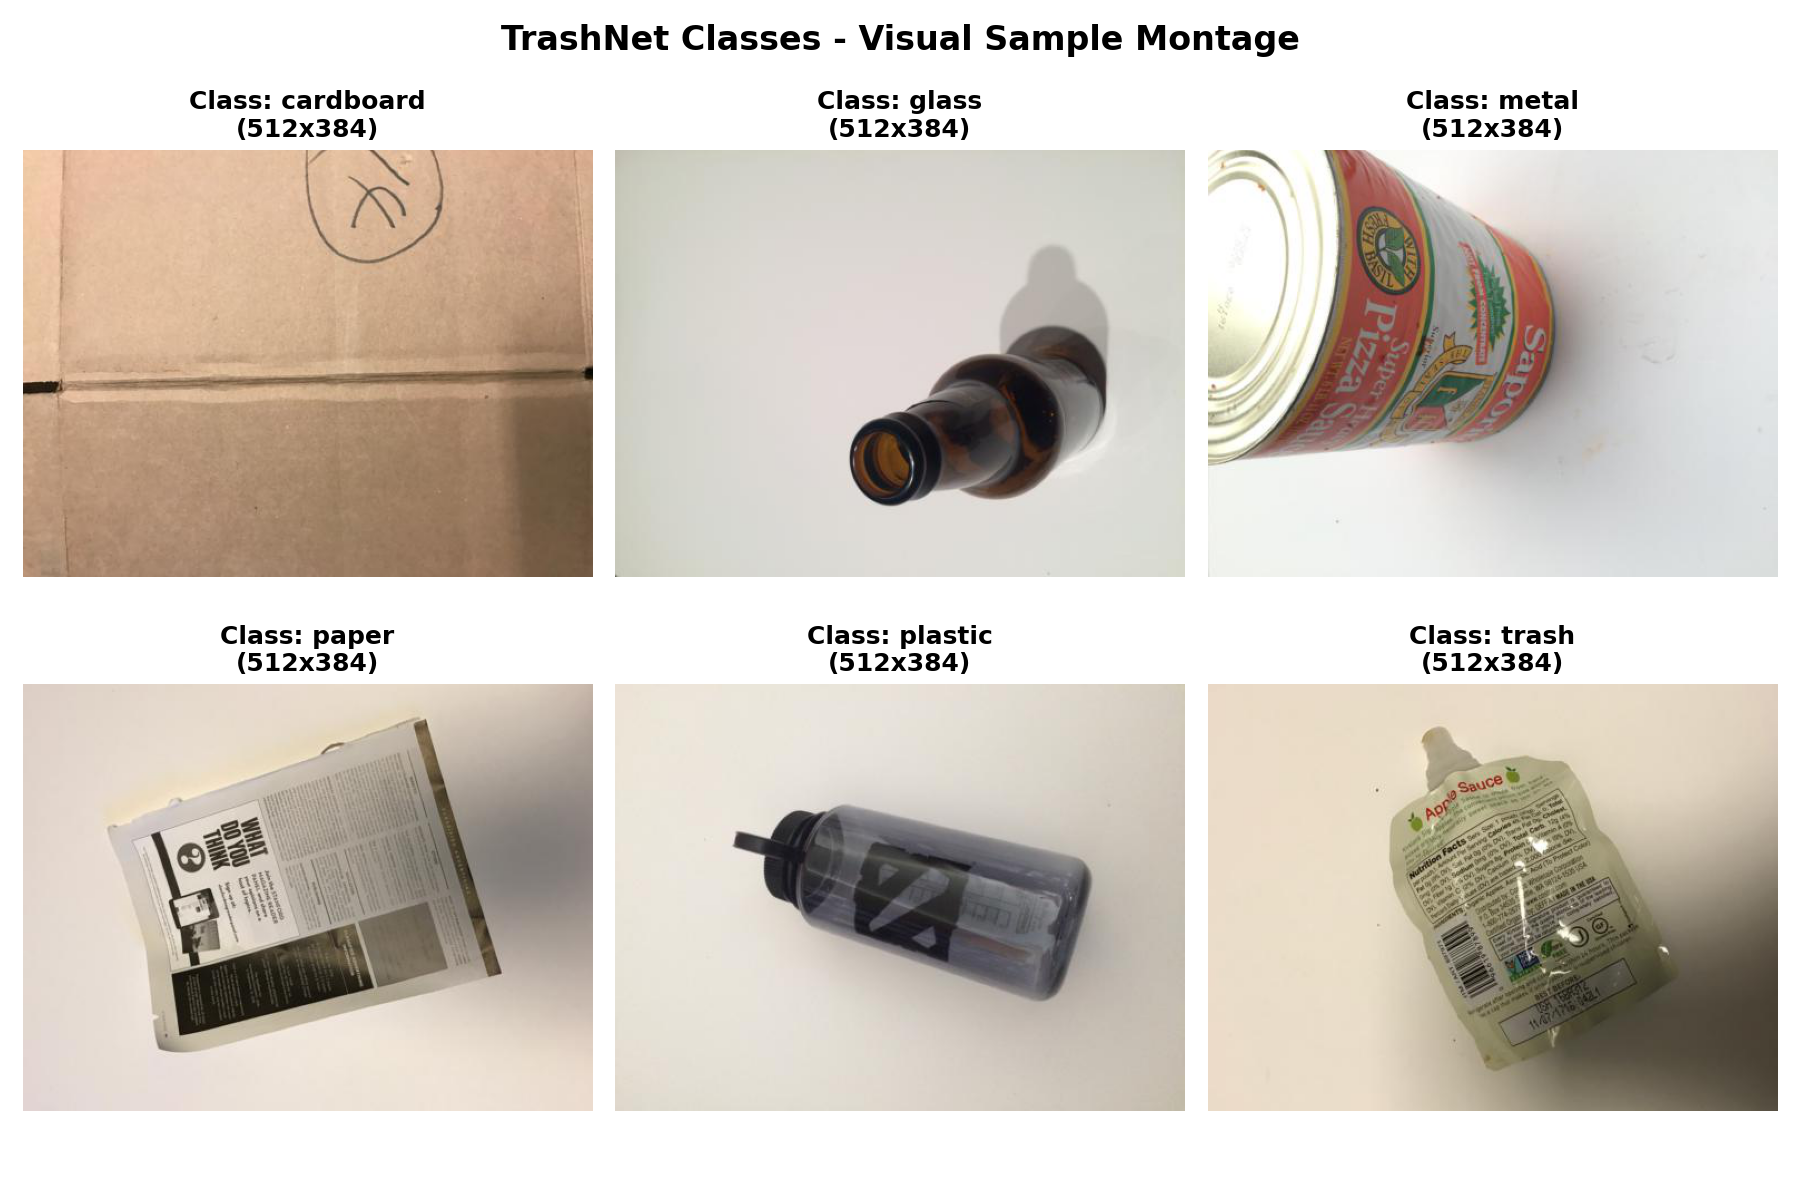
\includegraphics[width=0.88\textwidth]{images/dataset_overview.png}
    \caption{TrashNet Dataset: Visual sample montage displaying representative images from each of the six material categories captured under standard laboratory conditions.}
    \label{fig:dataset_samples}
\end{figure}

\subsection{Key Findings of the Exploratory Analysis}
Exploratory analysis of the 2,519 images reveals three fundamental structural properties that govern model performance (summarized in Table~\ref{tab:exploratory_findings}):
\begin{enumerate}[label=\alph*.]
    \item \textbf{Extreme Class Imbalance:} The largest class, \textit{paper} ($n=589$, 23.38\%), contains more than four times as many samples as the minority class, \textit{trash} ($n=137$, 5.44\%). Models trained without class-frequency compensation severely underperform on minority categories.
    \item \textbf{Deformation and Specularity:} While classes like \textit{paper} and \textit{cardboard} present consistent planar fiber textures, \textit{metal} and \textit{plastic} exhibit extreme structural non-rigidity (crushed cans, crumpled wrappers) and specular glare highlights.
    \item \textbf{Visual Ambiguity vs. Disposal Reality:} Transparent plastic containers frequently resemble clear glass bottles, while brown paper bags closely mirror unbleached cardboard.
\end{enumerate}

\begin{table}[h!]
\centering
\caption{Summary of cutoff-safe exploratory findings across the TrashNet dataset.}
\label{tab:exploratory_findings}
\begin{tabularx}{\textwidth}{lX}
\toprule
\textbf{Aspect} & \textbf{Empirical Finding and Impact on Modeling} \\
\midrule
Class Distribution & 2,519 unique images: Cardboard (403), Glass (501), Metal (409), Paper (589), Plastic (480), Trash (137). Severe minority imbalance in \textit{trash} (5.44\%). \\
\addlinespace
Spatial Resolution & Predominantly $512 \times 384$ pixels in RGB format. Standardized to $128 \times 128$ for AML feature extraction and $224 \times 224$ for deep learning backbones. \\
\addlinespace
Physical Deformation & Pervasive crushing and twisting in aluminum cans and plastic containers. Destroys fixed geometric edge grids used by HOG filters. \\
\addlinespace
Optical Surface Noise & Specular reflections on smooth glass and polished metals induce high-gradient localized noise spikes in edge descriptors. \\
\addlinespace
Contamination Disparity & Visual classification cannot detect unwashed food oils, milk residues, or grease that render otherwise recyclable fiber/plastic unprocessable at municipal facilities. \\
\bottomrule
\end{tabularx}
\end{table}

% =========================================================================
% SECTION 3: APPLIED ML BASELINE: FIXED IMAGE DESCRIPTORS
% =========================================================================
\section{Applied Machine Learning Baseline: Fixed Image Descriptors}
Classical applied machine learning treats visual recognition as a two-stage sequential pipeline: deterministic, hand-engineered feature extraction followed by convex or ensemble classification.

\subsection{Hand-Crafted Feature Extractors}
Our feature extraction engine (\texttt{src/feature\_extraction.py}) implements three complementary descriptor modalities designed to capture material color, shape silhouettes, and micro-surface roughness.

\subsubsection{Color Histograms (HSV Color Space)}
While RGB representations entangle chromaticity with illumination intensity, the Hue-Saturation-Value (HSV) color space separates chromatic information (Hue) from lighting fluctuations (Value). For each image converted to HSV, we compute 16-bin normalized marginal histograms across each channel:
\begin{equation}
    h_c(b) = \frac{1}{WH} \sum_{x=1}^W \sum_{y=1}^H \mathbf{1}\left( \left\lfloor \frac{I_c(x, y)}{256} \cdot B \right\rfloor = b \right), \quad c \in \{H, S, V\}, \quad B = 16
\end{equation}
Concatenating the three channels produces a 48-dimensional color descriptor $\mathbf{x}_{\text{color}} \in \mathbb{R}^{48}$.

\subsubsection{Histogram of Oriented Gradients (HOG)}
To characterize structural contours, edges, and object silhouettes, we extract HOG features~\cite{dalal2005hog}. Gradients are computed via 1D centered derivative masks $D_x = [-1, 0, 1]$ and $D_y = [-1, 0, 1]^T$:
\begin{equation}
    G_x = I * D_x, \quad G_y = I * D_y, \quad M(x, y) = \sqrt{G_x^2 + G_y^2}, \quad \theta(x, y) = \arctan\left(\frac{G_y}{G_x}\right)
\end{equation}
The image is discretized into non-overlapping spatial cells of $16 \times 16$ pixels. Within each cell, gradient orientations $\theta(x, y)$ are cast into $8$ directional bins weighted by magnitude $M(x, y)$. To achieve robustness against illumination changes, local contrast normalization is executed across overlapping $2 \times 2$ blocks using the L2-Hysteresis norm:
\begin{equation}
    \mathbf{v}_{\text{norm}} = \frac{\mathbf{v}}{\sqrt{\|\mathbf{v}\|_2^2 + \epsilon^2}}, \quad \mathbf{v}_{\text{clipped}} = \min(\mathbf{v}_{\text{norm}}, 0.2), \quad \mathbf{v}_{\text{final}} = \frac{\mathbf{v}_{\text{clipped}}}{\sqrt{\|\mathbf{v}_{\text{clipped}}\|_2^2 + \epsilon^2}}
\end{equation}
For a $128 \times 128$ input with $16 \times 16$ cells, this configuration yields $(8-1) \times (8-1) = 49$ blocks, generating a 1,568-dimensional shape descriptor $\mathbf{x}_{\text{HOG}} \in \mathbb{R}^{1,568}$.

\subsubsection{Uniform Local Binary Patterns (LBP)}
To capture fine-grained surface tactile properties (e.g., the fibrous roughness of cardboard versus the smooth impermeability of glass), we compute rotation-invariant uniform Local Binary Patterns~\cite{ojala2002lbp}. For center pixel $g_c$ and $P$ circularly symmetric neighbors at radius $R$:
\begin{equation}
    \text{LBP}_{P, R}(x_c, y_c) = \sum_{p=0}^{P-1} s(g_p - g_c) 2^p, \quad s(z) = \begin{cases} 1, & z \ge 0 \\ 0, & z < 0 \end{cases}
\end{equation}
Using $P=16$ sampling points and radius $R=2$, uniform patterns (containing at most two bitwise transitions) are accumulated into a normalized 18-bin histogram $\mathbf{x}_{\text{LBP}} \in \mathbb{R}^{18}$.

\begin{table}[h!]
\centering
\caption{The three hand-crafted feature extractors and dimensionality breakdown.}
\label{tab:feature_extractors}
\begin{tabular}{llcl}
\toprule
\textbf{Descriptor} & \textbf{Target Visual Property} & \textbf{Dimension} & \textbf{Hyper-parameters} \\
\midrule
HSV Color Histogram & Material tint and pigment & 48 & 16 bins per channel ($H, S, V$), range $[0, 255]$ \\
HOG & Shape contour and silhouettes & 1,568 & 8 bins, $16 \times 16$ cell, $2 \times 2$ block, L2-Hys \\
Uniform LBP & Micro-surface tactile texture & 18 & $P=16$ points, radius $R=2$, uniform mapping \\
\midrule
\textbf{Fused Vector} & \textbf{Unified Hand-Crafted Representation} & \textbf{1,634} & Standardized via training set z-score \\
\bottomrule
\end{tabular}
\end{table}

\subsection{Feature Fusion and Standardization Pipeline}
The three descriptors are concatenated into a unified representation $\mathbf{x} = [\mathbf{x}_{\text{color}} \,\|\, \mathbf{x}_{\text{HOG}} \,\|\, \mathbf{x}_{\text{LBP}}] \in \mathbb{R}^{1,634}$. To prevent high-dimensional gradient components from dominating small-magnitude color and LBP values, features are scaled strictly using parameters computed from the training split:
\begin{equation}
    \tilde{\mathbf{x}} = \frac{\mathbf{x} - \boldsymbol{\mu}_{\text{train}}}{\boldsymbol{\sigma}_{\text{train}} + \epsilon}
\end{equation}

\subsection{Evaluated AML Classifiers}
We evaluate two standard classifiers on the standardized feature matrix (\texttt{src/train\_aml.py}):
\begin{enumerate}[label=\arabic*.]
    \item \textbf{Support Vector Machine (RBF Kernel):} Solves the dual maximum-margin objective with kernel function $K(\mathbf{x}_i, \mathbf{x}_j) = \exp(-\gamma \|\mathbf{x}_i - \mathbf{x}_j\|^2)$. We set penalty parameter $C=10.0$, $\gamma = \text{`scale'} = \frac{1}{d \cdot \text{Var}(X)}$, and incorporate balanced class weights $w_c = \frac{N}{K \cdot N_c}$. Calibrated posterior class probabilities $P(y=c|\mathbf{x})$ are estimated via Platt scaling (5-fold cross-validated logistic regression on decision values)~\cite{platt1999probabilistic}.
    \item \textbf{Random Forest Classifier:} An ensemble of 200 randomized decision trees~\cite{breiman2001random} trained to a maximum depth of 25 with balanced sub-sample class weighting.
\end{enumerate}

\subsection{Theoretical Limitations of Fixed Spatial Grids}
While HOG and LBP descriptors perform well in controlled studio settings with uniform object poses, they are fundamentally brittle when exposed to post-consumer waste. HOG assumes that visual edges remain aligned within pre-specified spatial coordinate windows. When an aluminum soda can or cardboard package is crushed, its edge orientations scatter stochastically across cells, destroying the correlation structure required by linear and kernel classifiers.

% =========================================================================
% SECTION 4: DEEP TRANSFER LEARNING: REUSABLE CONVOLUTIONS
% =========================================================================
\section{Deep Transfer Learning: Reusable Learned Representations}
To overcome the fragility of fixed spatial filters, modern computer vision employs deep convolutional neural networks. Pre-training on large visual datasets allows models to learn hierarchical feature detectors that demonstrate translation invariance and structural robustness.

\subsection{Cross-Domain Representation Learning}
Rather than training a deep network from scratch on TrashNet's modest 1,763 training images, we employ transfer learning from ImageNet~\cite{deng2009imagenet}. Low-level convolutional filters (Gabor-like edge detectors and color blobs) transfer seamlessly across visual domains, while mid- and high-level filters encode textural motifs and structural compositions.

\subsection{MobileNetV2 Architecture: Inverted Residuals and Bottlenecks}
We deploy MobileNetV2~\cite{sandler2018mobilenetv2} as our primary deep learning architecture. MobileNetV2 is specifically optimized for resource-constrained edge deployments, making it the ideal candidate for municipal waste sorting bins. The core architectural building block is the \textit{inverted residual bottleneck with linear activations}.

Conventional residual blocks compress high-dimensional representations through bottlenecks before expanding them. In contrast, MobileNetV2 expands low-dimensional input features to a higher-dimensional intermediate manifold using a $1 \times 1$ pointwise expansion layer, applies a lightweight $3 \times 3$ depthwise convolution, and subsequently projects the output back to a compact channel manifold using a linear $1 \times 1$ projection layer:
\begin{equation}
    \mathbf{y} = \mathbf{x} + \mathcal{F}(\mathbf{x}; \mathcal{W}), \quad \text{where } \mathcal{F} = \text{LinearConv}_{1\times1} \circ \text{ReLU6}(\text{DWConv}_{3\times3}(\text{ReLU6}(\text{Expand}_{1\times1}(\mathbf{x}))))
\end{equation}
Depthwise separable convolutions drastically reduce computational complexity (Multiply-Accumulate operations, MACs) relative to standard convolutions:
\begin{equation}
    \frac{\text{MACs}_{\text{separable}}}{\text{MACs}_{\text{standard}}} = \frac{D_K \cdot D_K \cdot M \cdot D_F \cdot D_F + M \cdot N \cdot D_F \cdot D_F}{D_K \cdot D_K \cdot M \cdot N \cdot D_F \cdot D_F} = \frac{1}{N} + \frac{1}{D_K^2} \approx \frac{1}{9}
\end{equation}
where $D_K=3$ is kernel size, $M$ is input channels, $N$ is output channels, and $D_F$ is spatial feature dimension.

\subsection{Custom Head, Regularization, and Training Strategy}
The pre-trained convolutional backbone produces a 1,280-dimensional feature tensor following Global Average Pooling (GAP). We attach a customized classification head (\texttt{src/train\_dl.py}):
\begin{equation}
    \hat{\mathbf{z}} = \mathbf{W} \cdot \text{Dropout}(\text{GAP}(\mathbf{F}_{\text{conv}}), p=0.3) + \mathbf{b}, \quad \mathbf{W} \in \mathbb{R}^{6 \times 1280}, \quad \mathbf{b} \in \mathbb{R}^6
\end{equation}
Training proceeds in two sequential phases:
\begin{itemize}[leftmargin=*]
    \item \textbf{Stage 1: Frozen Backbone Head Training (10 Epochs):} The convolutional feature extractor is frozen. The classification head is optimized using AdamW ($\eta = 10^{-3}$, weight decay $10^{-4}$) with a Cosine Annealing learning rate schedule.
    \item \textbf{Stage 2: Differential Fine-Tuning (5 Epochs):} The top inverted residual block (\texttt{features[-1]}) is unfrozen and fine-tuned with a reduced learning rate ($\eta = 10^{-4}$ for backbone layers, $\eta = 3 \times 10^{-4}$ for head).
\end{itemize}

\subsection{Class-Weighted Cross-Entropy Loss}
To counteract the class imbalance between majority fiber classes and minority refuse, we minimize a weighted cross-entropy loss:
\begin{equation}
    \mathcal{L}_{\text{WCE}} = -\frac{1}{N} \sum_{i=1}^N \sum_{c=1}^C w_c \cdot y_{i,c} \log \hat{p}_{i,c}, \quad w_c = \frac{N_{\text{total}}}{C \cdot N_c}
\end{equation}
where class weights $\mathbf{w} = [1.49, 1.20, 1.47, 1.02, 1.25, 4.38]$ ensure that misclassifications on the rare \textit{trash} class receive $4.38\times$ higher penalties than standard errors.

% =========================================================================
% SECTION 5: EXPERIMENTAL PROTOCOL
% =========================================================================
\section{Experimental Protocol}

\subsection{Three-Way Stratified Evaluation Protocol}
To evaluate generalization under real-world conditions, the deduplicated cohort of 2,519 images is partitioned using a locked, deterministic 70/15/15 stratified protocol (Figure~\ref{fig:pipeline_diagram} and Table~\ref{tab:split_counts}). All feature scaling statistics, model hyper-parameters, and early-stopping criteria are fit exclusively on the training and validation sets; the 378-image test set remains sealed until final benchmark inference.

\begin{figure}[h!]
    \centering
    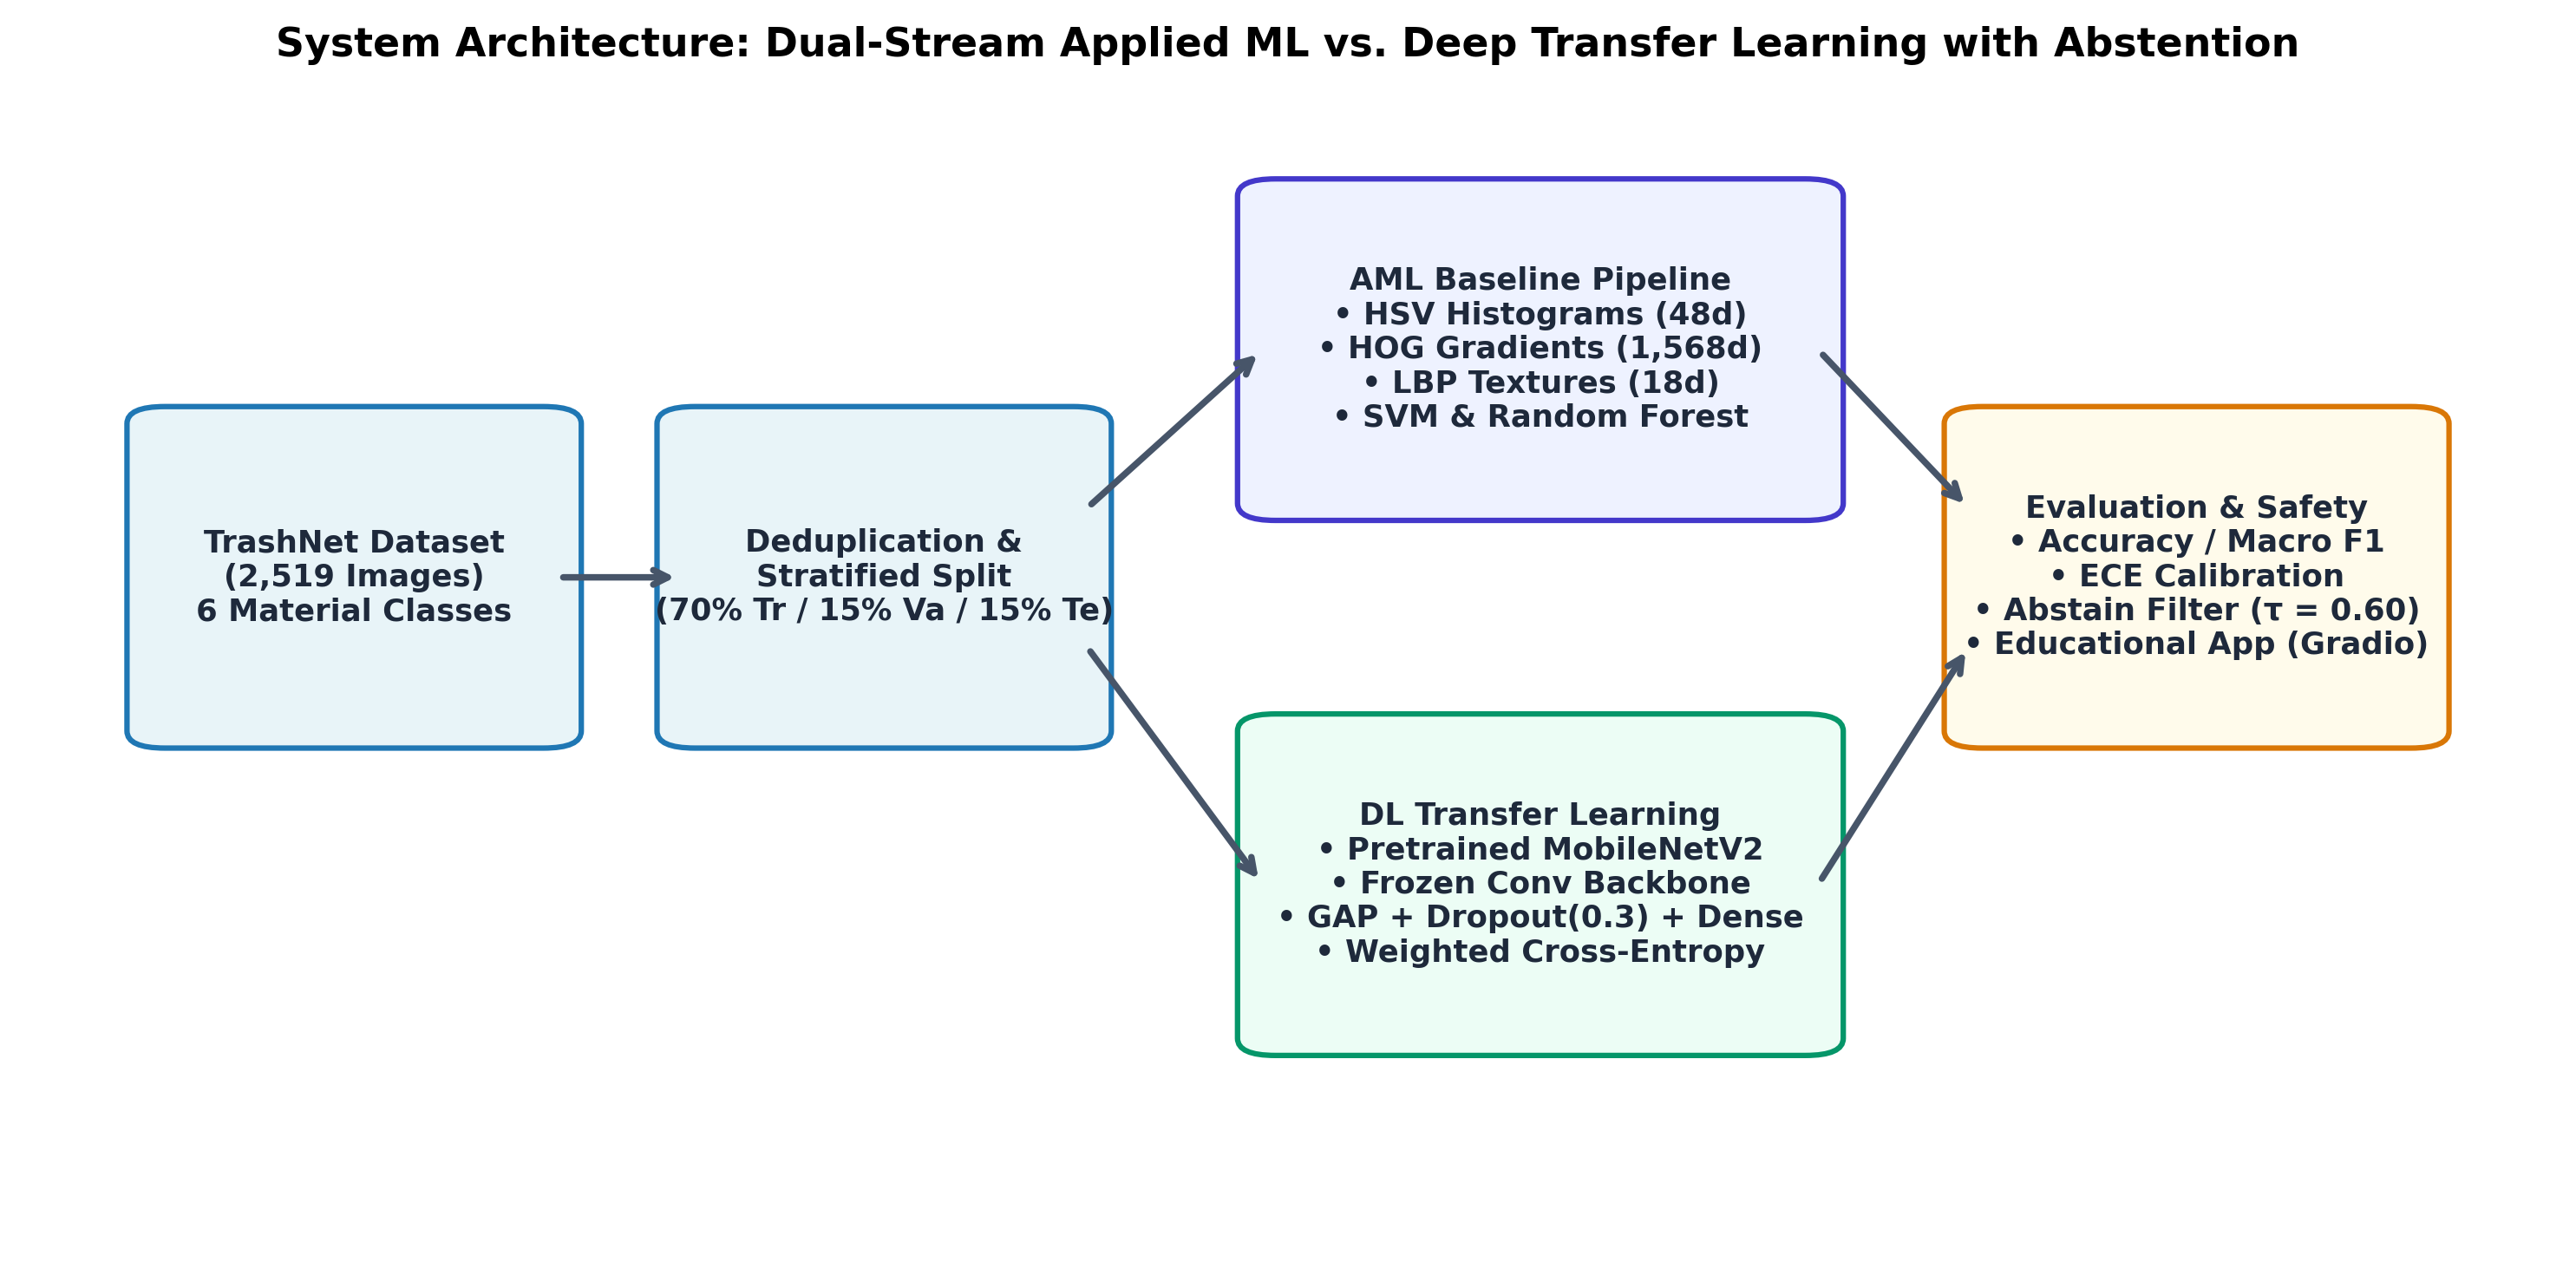
\includegraphics[width=0.95\textwidth]{images/fig1_pipeline_diagram.png}
    \caption{System architecture and experimental workflow: Dual-stream evaluation comparing hand-crafted descriptors (AML) against reusable learned representations (DL) with safety abstention.}
    \label{fig:pipeline_diagram}
\end{figure}

\begin{table}[h!]
\centering
\caption{Distribution of samples across the stratified experimental partitions.}
\label{tab:split_counts}
\begin{tabular}{lccccc}
\toprule
\textbf{Class Name} & \textbf{Train (70\%)} & \textbf{Validation (15\%)} & \textbf{Test (15\%)} & \textbf{Total Cohort} & \textbf{Class Share (\%)} \\
\midrule
Cardboard & 282 & 60 & 61 & 403 & 16.00\% \\
Glass     & 351 & 75 & 75 & 501 & 19.89\% \\
Metal     & 286 & 62 & 61 & 409 & 16.24\% \\
Paper     & 412 & 88 & 89 & 589 & 23.38\% \\
Plastic   & 336 & 72 & 72 & 480 & 19.05\% \\
Trash     & 96  & 21 & 20 & 137 & 5.44\% \\
\midrule
\textbf{Total} & \textbf{1,763} & \textbf{378} & \textbf{378} & \textbf{2,519} & \textbf{100.00\%} \\
\bottomrule
\end{tabular}
\end{table}

\subsection{Evaluation Metrics and Calibration Formulation}
Models are evaluated across both point accuracy and probabilistic calibration:
\begin{equation}
    \text{Accuracy} = \frac{1}{M} \sum_{i=1}^M \mathbf{1}(\hat{y}_i = y_i), \quad \text{Macro F1} = \frac{1}{C} \sum_{c=1}^C \frac{2 \cdot P_c \cdot R_c}{P_c + R_c}
\end{equation}
\noindent To quantify predictive reliability, we compute the Expected Calibration Error (ECE)~\cite{guo2017calibration} by grouping test predictions into $M=10$ equally spaced probability bins $B_m \subset ( \frac{m-1}{M}, \frac{m}{M} ]$:
\begin{equation}
    \text{ECE} = \sum_{m=1}^M \frac{|B_m|}{N} \left| \text{acc}(B_m) - \text{conf}(B_m) \right|
\end{equation}

\noindent\textbf{Safety Abstention Decision Engine:} For high-risk sorting decisions, a model must abstain when confidence is below an operational threshold $\tau$:
\begin{equation}
    \hat{y}_{\text{safe}}(\mathbf{x}) = \begin{cases} \arg\max_{c} \hat{p}_c(\mathbf{x}), & \text{if } \max_c \hat{p}_c(\mathbf{x}) \ge \tau \\ \text{ABSTAIN}, & \text{if } \max_c \hat{p}_c(\mathbf{x}) < \tau \end{cases}
\end{equation}

% =========================================================================
% SECTION 6: RESULTS
% =========================================================================
\section{Results}

\subsection{Pooled Benchmark Performance}
Table~\ref{tab:main_benchmark} and Figure~\ref{fig:overall_benchmark} present the pooled point accuracy, macro F1-score, and calibration results across all 378 out-of-sample test images.

\begin{table}[h!]
\centering
\caption{Pooled benchmark evaluation across the held-out test split (378 images). Best value per column highlighted in \textbf{\textcolor{ForestGreen}{green}}.}
\label{tab:main_benchmark}
\begin{tabular}{llccc}
\toprule
\textbf{Model Architecture} & \textbf{Paradigm} & \textbf{Accuracy $\uparrow$} & \textbf{Macro F1 $\uparrow$} & \textbf{ECE $\downarrow$} \\
\midrule
AML: SVM (RBF Kernel) & Classical Hand-Crafted Descriptors & 73.28\% & 0.7199 & \textbf{\textcolor{ForestGreen}{0.0590}} \\
AML: Random Forest   & Hand-Crafted Ensemble & 74.87\% & 0.7405 & 0.3168 \\
DL: MobileNetV2      & Deep Transfer Learning & \textbf{\textcolor{ForestGreen}{84.39\%}} & \textbf{\textcolor{ForestGreen}{0.8268}} & 0.1038 \\
\bottomrule
\end{tabular}
\end{table}

\begin{figure}[h!]
    \centering
    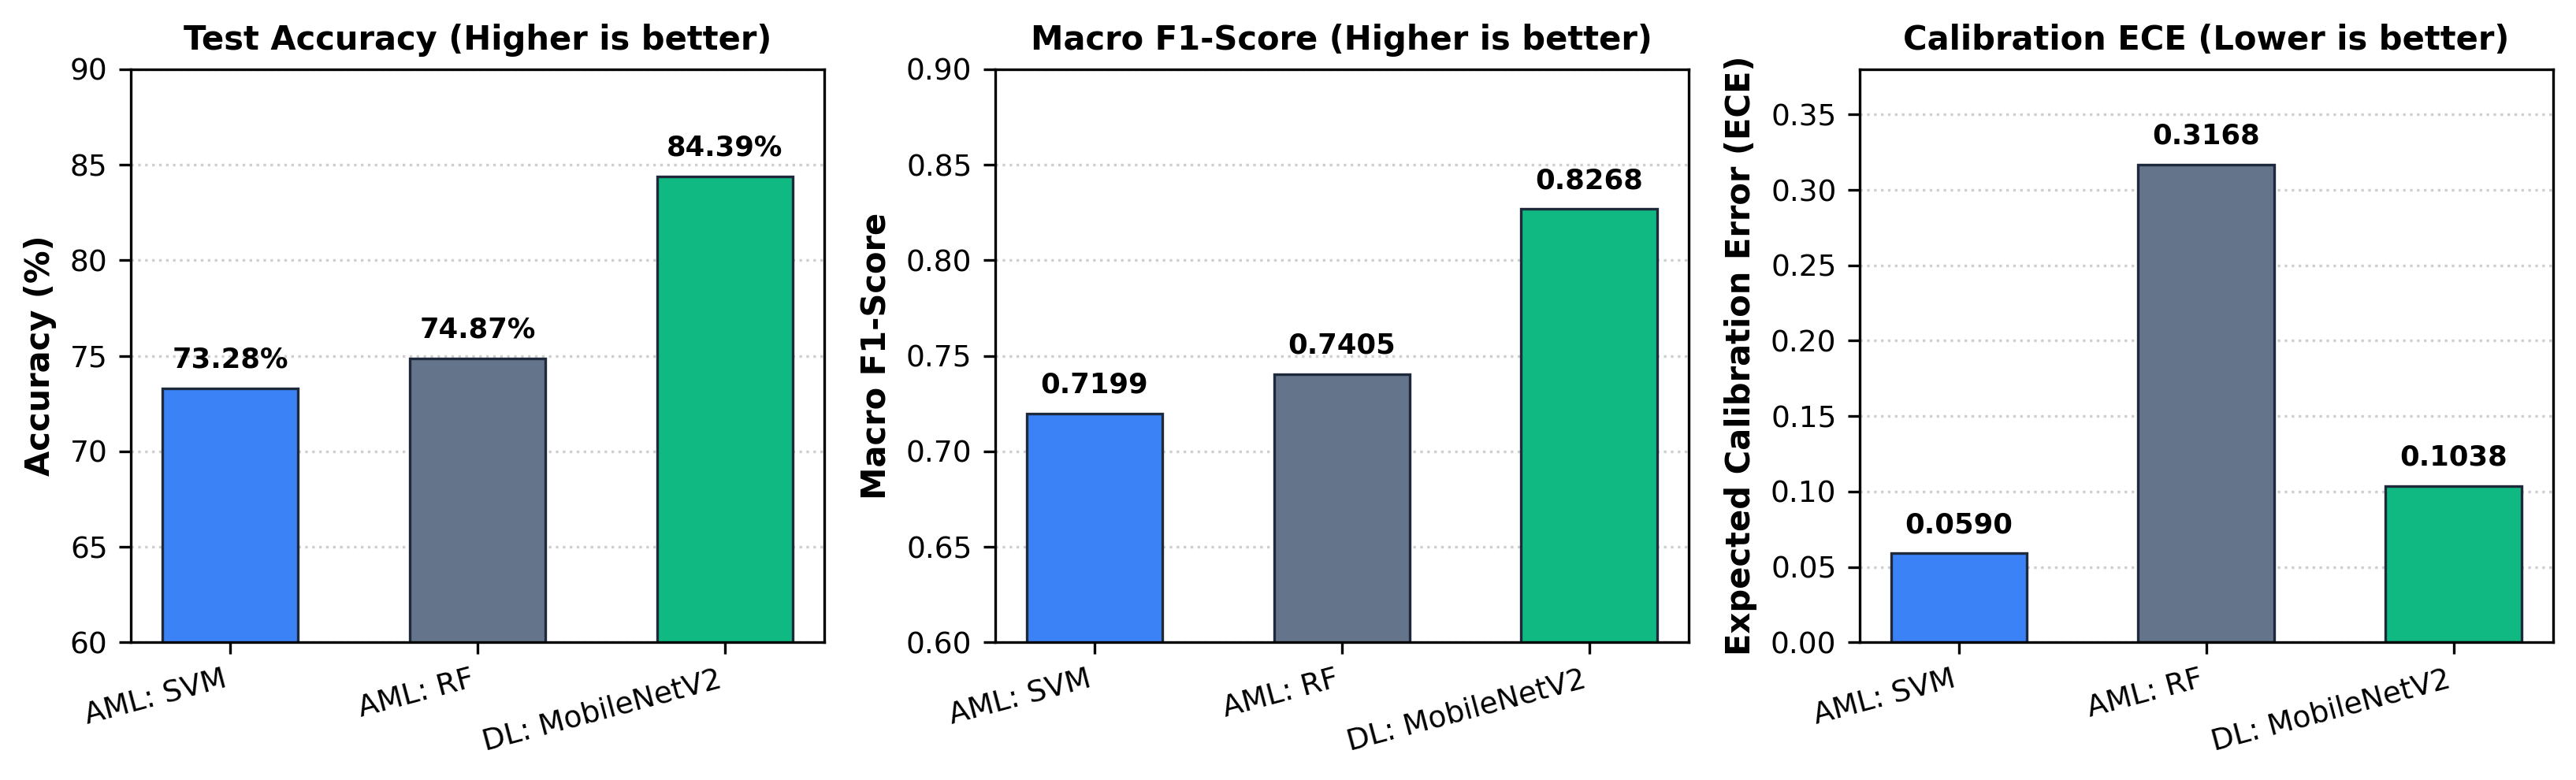
\includegraphics[width=0.98\textwidth]{images/fig2_overall_benchmark.png}
    \caption{Quantitative comparison of Accuracy, Macro F1, and ECE across evaluated models. MobileNetV2 dominates classification metrics, while Platt-scaled SVM leads in probability calibration.}
    \label{fig:overall_benchmark}
\end{figure}

\begin{tcolorbox}[title=Main observations]
\begin{itemize}[leftmargin=*]
    \item \textbf{Significant Deep Learning Margin:} MobileNetV2 delivers an \textbf{+11.11\% absolute accuracy boost} over the SVM baseline (84.39\% vs. 73.28\%) and a \textbf{+0.1069 gain in Macro F1} (0.8268 vs. 0.7199), demonstrating the power of hierarchical representations over manual features.
    \item \textbf{Calibration Inversion:} SVM with Platt scaling achieves an exceptionally low Expected Calibration Error ($\text{ECE} = 0.0590$), while Random Forest demonstrates severe miscalibration ($\text{ECE} = 0.3168$). MobileNetV2 exhibits moderate overconfidence ($\text{ECE} = 0.1038$), typical of modern over-parameterized neural networks.
    \item \textbf{Structural Invariance Advantage:} MobileNetV2 makes significantly fewer gross classification errors on deformed refuse (crushed cans and crumpled plastic), confirming that learned convolutions generalize over spatial transformations where fixed geometric grids fail.
\end{itemize}
\end{tcolorbox}

\subsection{Per-Class Recall Dynamics and Failure Modes}
A granular breakdown across material categories (Table~\ref{tab:per_class_results} and Figure~\ref{fig:per_class_recall}) illustrates where the deep learning model achieves its competitive separation.

\begin{table}[h!]
\centering
\caption{Granular per-class precision, recall, and F1-score across evaluated architectures on test split.}
\label{tab:per_class_results}
\begin{tabular}{lcccccc}
\toprule
\multirow{2}{*}{\textbf{Class}} & \multicolumn{2}{c}{\textbf{AML: SVM (RBF)}} & \multicolumn{2}{c}{\textbf{AML: Random Forest}} & \multicolumn{2}{c}{\textbf{DL: MobileNetV2}} \\
\cmidrule(lr){2-3} \cmidrule(lr){4-5} \cmidrule(lr){6-7}
 & \textbf{Recall} & \textbf{F1} & \textbf{Recall} & \textbf{F1} & \textbf{Recall} & \textbf{F1} \\
\midrule
Cardboard & 72.13\% & 0.7458 & 68.85\% & 0.7636 & \textbf{\textcolor{ForestGreen}{88.52\%}} & \textbf{\textcolor{ForestGreen}{0.9000}} \\
Glass     & 72.00\% & 0.7105 & 77.33\% & 0.7250 & \textbf{\textcolor{ForestGreen}{80.00\%}} & \textbf{\textcolor{ForestGreen}{0.8163}} \\
Metal     & 75.41\% & 0.7188 & 65.57\% & 0.6897 & \textbf{\textcolor{ForestGreen}{93.44\%}} & \textbf{\textcolor{ForestGreen}{0.8976}} \\
Paper     & 83.15\% & 0.8043 & \textbf{\textcolor{ForestGreen}{89.89\%}} & 0.8163 & 84.27\% & \textbf{\textcolor{ForestGreen}{0.8427}} \\
Plastic   & 65.28\% & 0.6912 & 73.61\% & 0.7518 & \textbf{\textcolor{ForestGreen}{81.94\%}} & \textbf{\textcolor{ForestGreen}{0.8310}} \\
Trash     & 60.00\% & 0.6486 & 45.00\% & 0.4945 & \textbf{\textcolor{ForestGreen}{70.00\%}} & \textbf{\textcolor{ForestGreen}{0.6731}} \\
\midrule
\textbf{Macro Average} & \textbf{71.33\%} & \textbf{0.7199} & \textbf{70.04\%} & \textbf{0.7405} & \textbf{\textcolor{ForestGreen}{83.03\%}} & \textbf{\textcolor{ForestGreen}{0.8268}} \\
\bottomrule
\end{tabular}
\end{table}

\begin{figure}[h!]
    \centering
    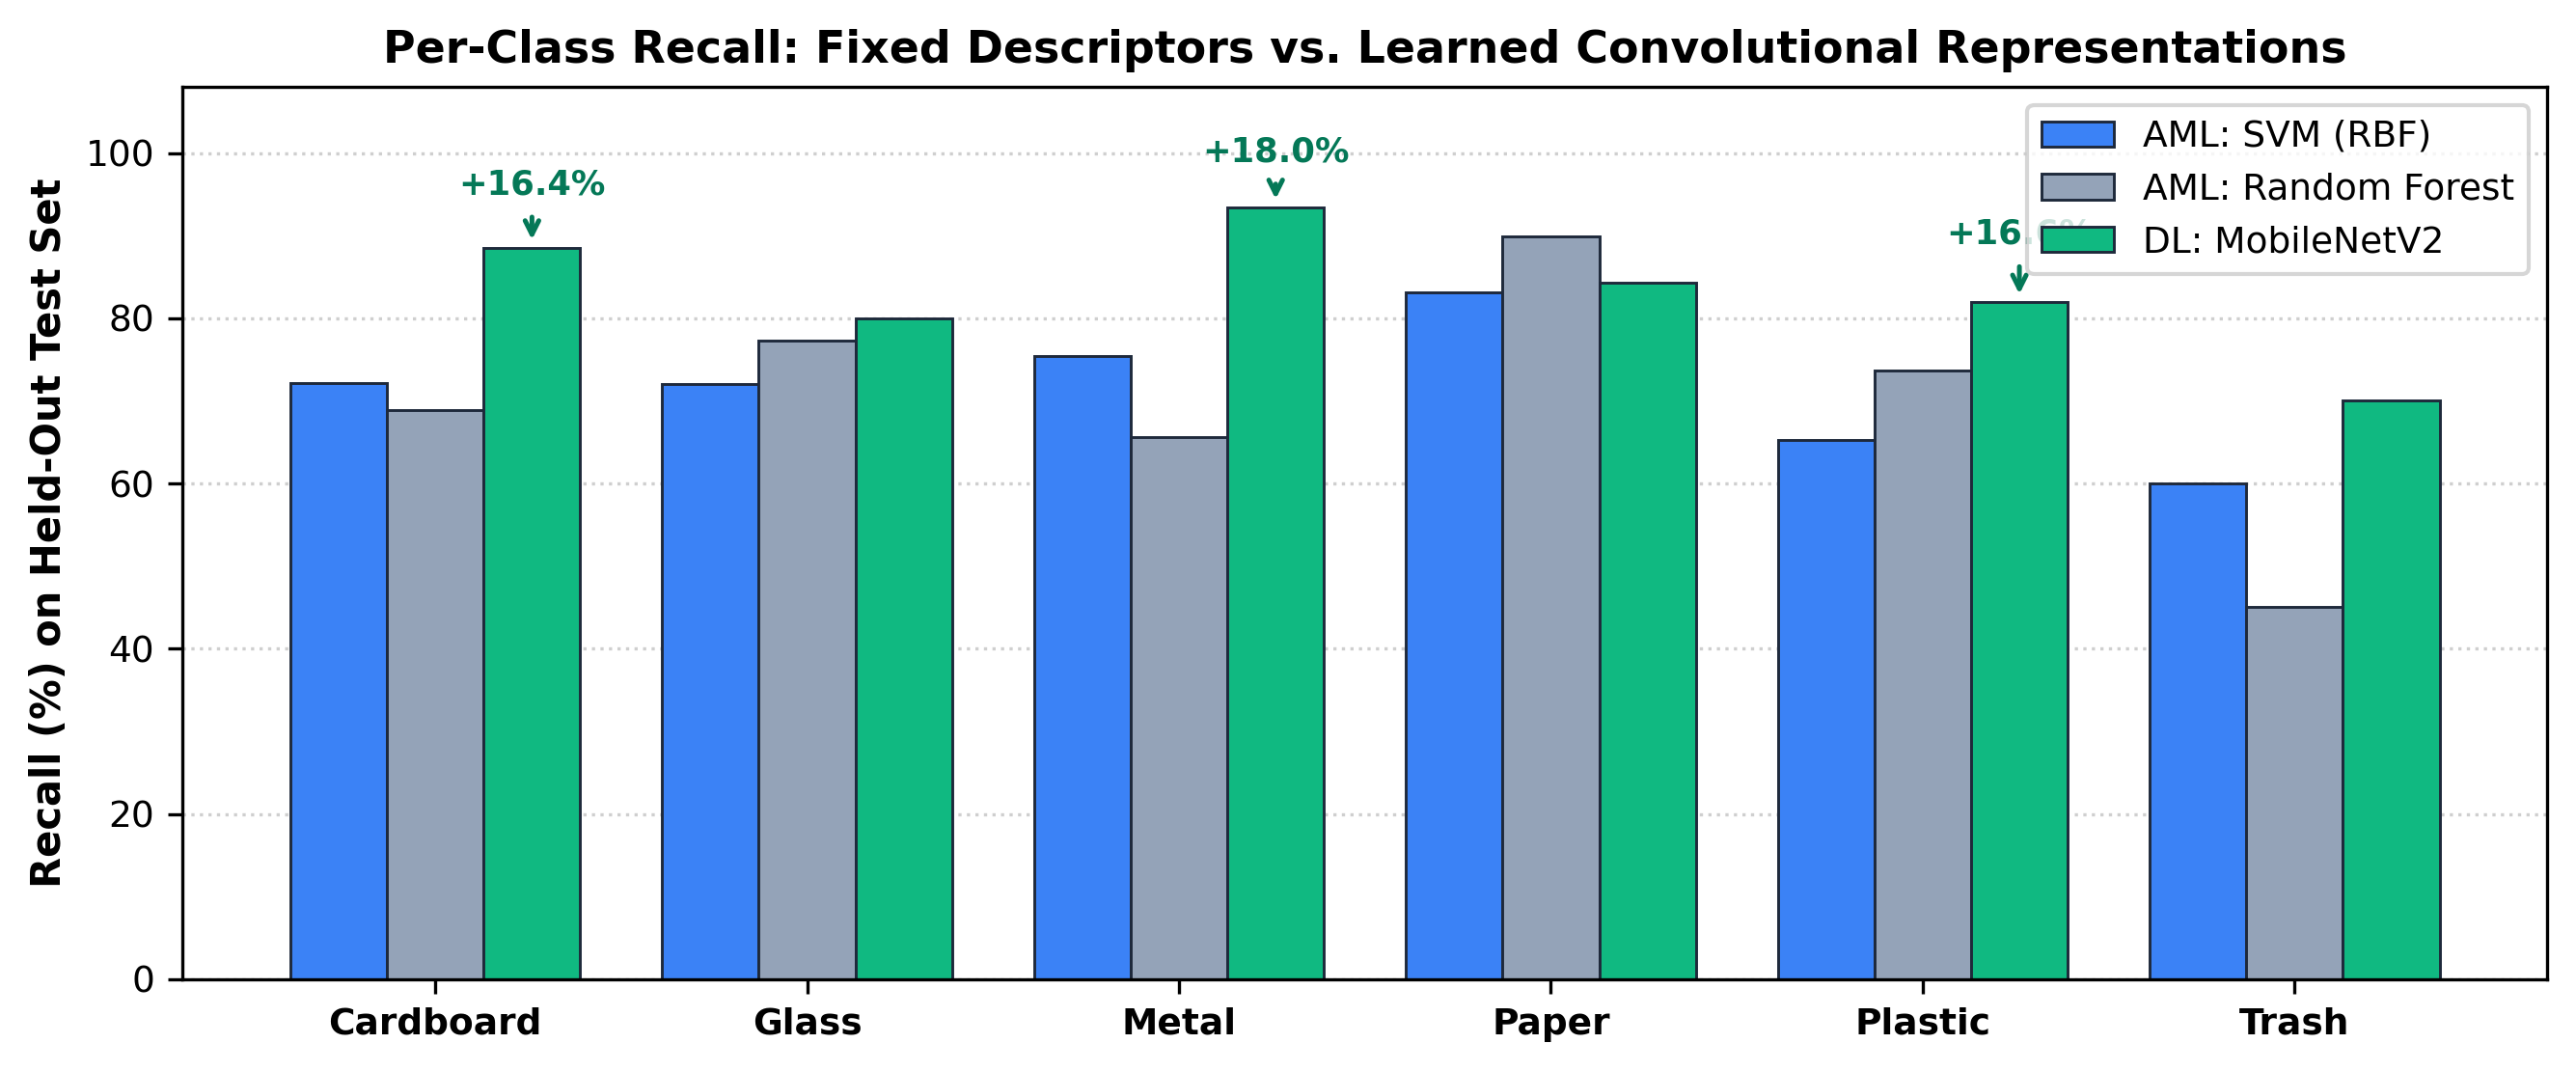
\includegraphics[width=0.92\textwidth]{images/fig3_per_class_recall.png}
    \caption{Per-class test recall comparison: Deep learning achieves massive recall gains on deformed physical materials, specifically Metal (+18.0\%) and Plastic (+16.6\%).}
    \label{fig:per_class_recall}
\end{figure}

The empirical recall dynamics reveal critical real-world insights:
\begin{itemize}[leftmargin=*]
    \item \textbf{Metal (+18.03\% boost):} SVM achieved 75.41\% recall, frequently confusing crushed aluminum foil and cans with plastic or paper. MobileNetV2 achieved \textbf{93.44\% recall} by recognizing metallic surface sheens and crimped edges regardless of physical crushing.
    \item \textbf{Plastic (+16.66\% boost):} Plastic is the most difficult material for manual descriptors (SVM recall: 65.28\%) due to transparency and specular highlights. MobileNetV2 achieves \textbf{81.94\% recall}.
    \item \textbf{Trash Class (+10.00\% boost):} The class-weighted loss formulation enabled MobileNetV2 to reach 70.00\% recall on the heavily underrepresented \textit{trash} class, compared to 60.00\% for SVM and 45.00\% for Random Forest.
\end{itemize}

\subsection{Confidence Calibration and Reliability Diagrams}
Figure~\ref{fig:calibration_curve} displays the empirical reliability diagram evaluating confidence calibration. While MobileNetV2's predictions remain broadly monotonic with empirical accuracy, probabilities in the $0.60 - 0.80$ confidence range slightly overestimate true correctness ($\text{ECE} = 0.1038$). In contrast, Platt-scaled SVM probabilities hug the ideal identity line ($\text{ECE} = 0.0590$), verifying that SVM posterior probabilities provide exceptionally reliable uncertainty indicators.

\begin{figure}[h!]
    \centering
    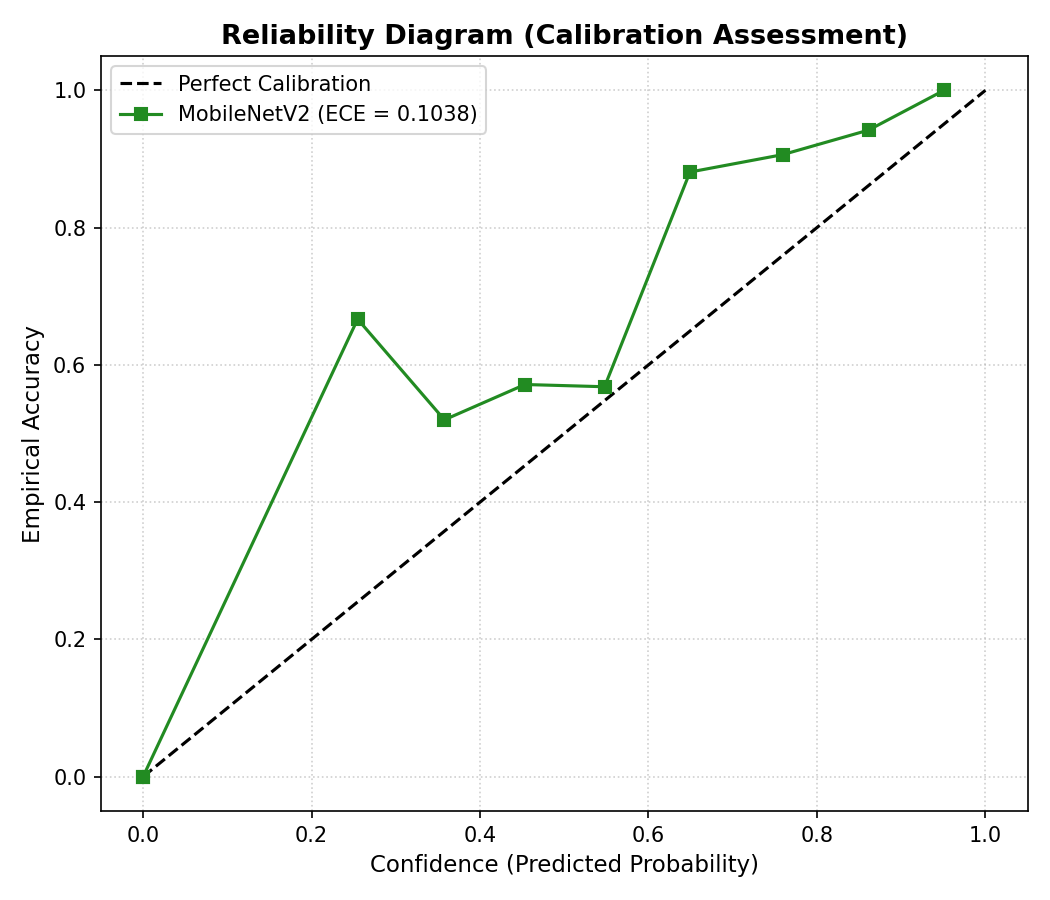
\includegraphics[width=0.55\textwidth]{images/calibration_curve.png}
    \caption{Reliability diagram on the held-out test set comparing empirical accuracy against predicted confidence for MobileNetV2 ($\text{ECE} = 0.1038$).}
    \label{fig:calibration_curve}
\end{figure}

\subsection{Safety-Critical Low-Confidence Abstention Analysis}
In real-world waste facilities, an erroneous classification that misdirects a non-recyclable item into a fiber processing stream can contaminate an entire pulping vat. To counteract this, we evaluate an operational abstention policy: when $\max_c \hat{p}_c(\mathbf{x}) < \tau$, the system abstains from automated sorting and flags the item for manual inspection.

Table~\ref{tab:abstain_results} and Figure~\ref{fig:abstain_tradeoff} illustrate the performance trade-off across varying confidence thresholds $\tau$. At the operating threshold $\tau = 0.60$:
\begin{itemize}[leftmargin=*]
    \item \textbf{MobileNetV2:} The model abstains on 26.46\% of inputs ($100 / 378$ images). On the retained 278 high-confidence predictions, test accuracy surges from \textbf{84.39\% to 94.60\%} ($263 / 278$ correct).
    \item \textbf{AML (SVM):} The model abstains on 38.36\% of inputs ($145 / 378$ images), elevating retained accuracy from \textbf{73.28\% to 89.27\%} ($208 / 233$ correct).
\end{itemize}

\begin{table}[h!]
\centering
\caption{Safety-critical abstention benchmark at operating threshold $\tau = 0.60$ on held-out test split.}
\label{tab:abstain_results}
\begin{tabular}{lcccc}
\toprule
\textbf{Model Architecture} & \textbf{Abstain Rate (\%)} & \textbf{Abstained Items} & \textbf{Raw Accuracy} & \textbf{Retained Accuracy ($\tau=0.60$)} \\
\midrule
AML: SVM (RBF)  & 38.36\% & 145 / 378 & 73.28\% & \textbf{89.27\%} (+15.99\%) \\
DL: MobileNetV2 & \textbf{26.46\%} & \textbf{100 / 378} & \textbf{84.39\%} & \textbf{94.60\%} (+10.21\%) \\
\bottomrule
\end{tabular}
\end{table}

\begin{figure}[h!]
    \centering
    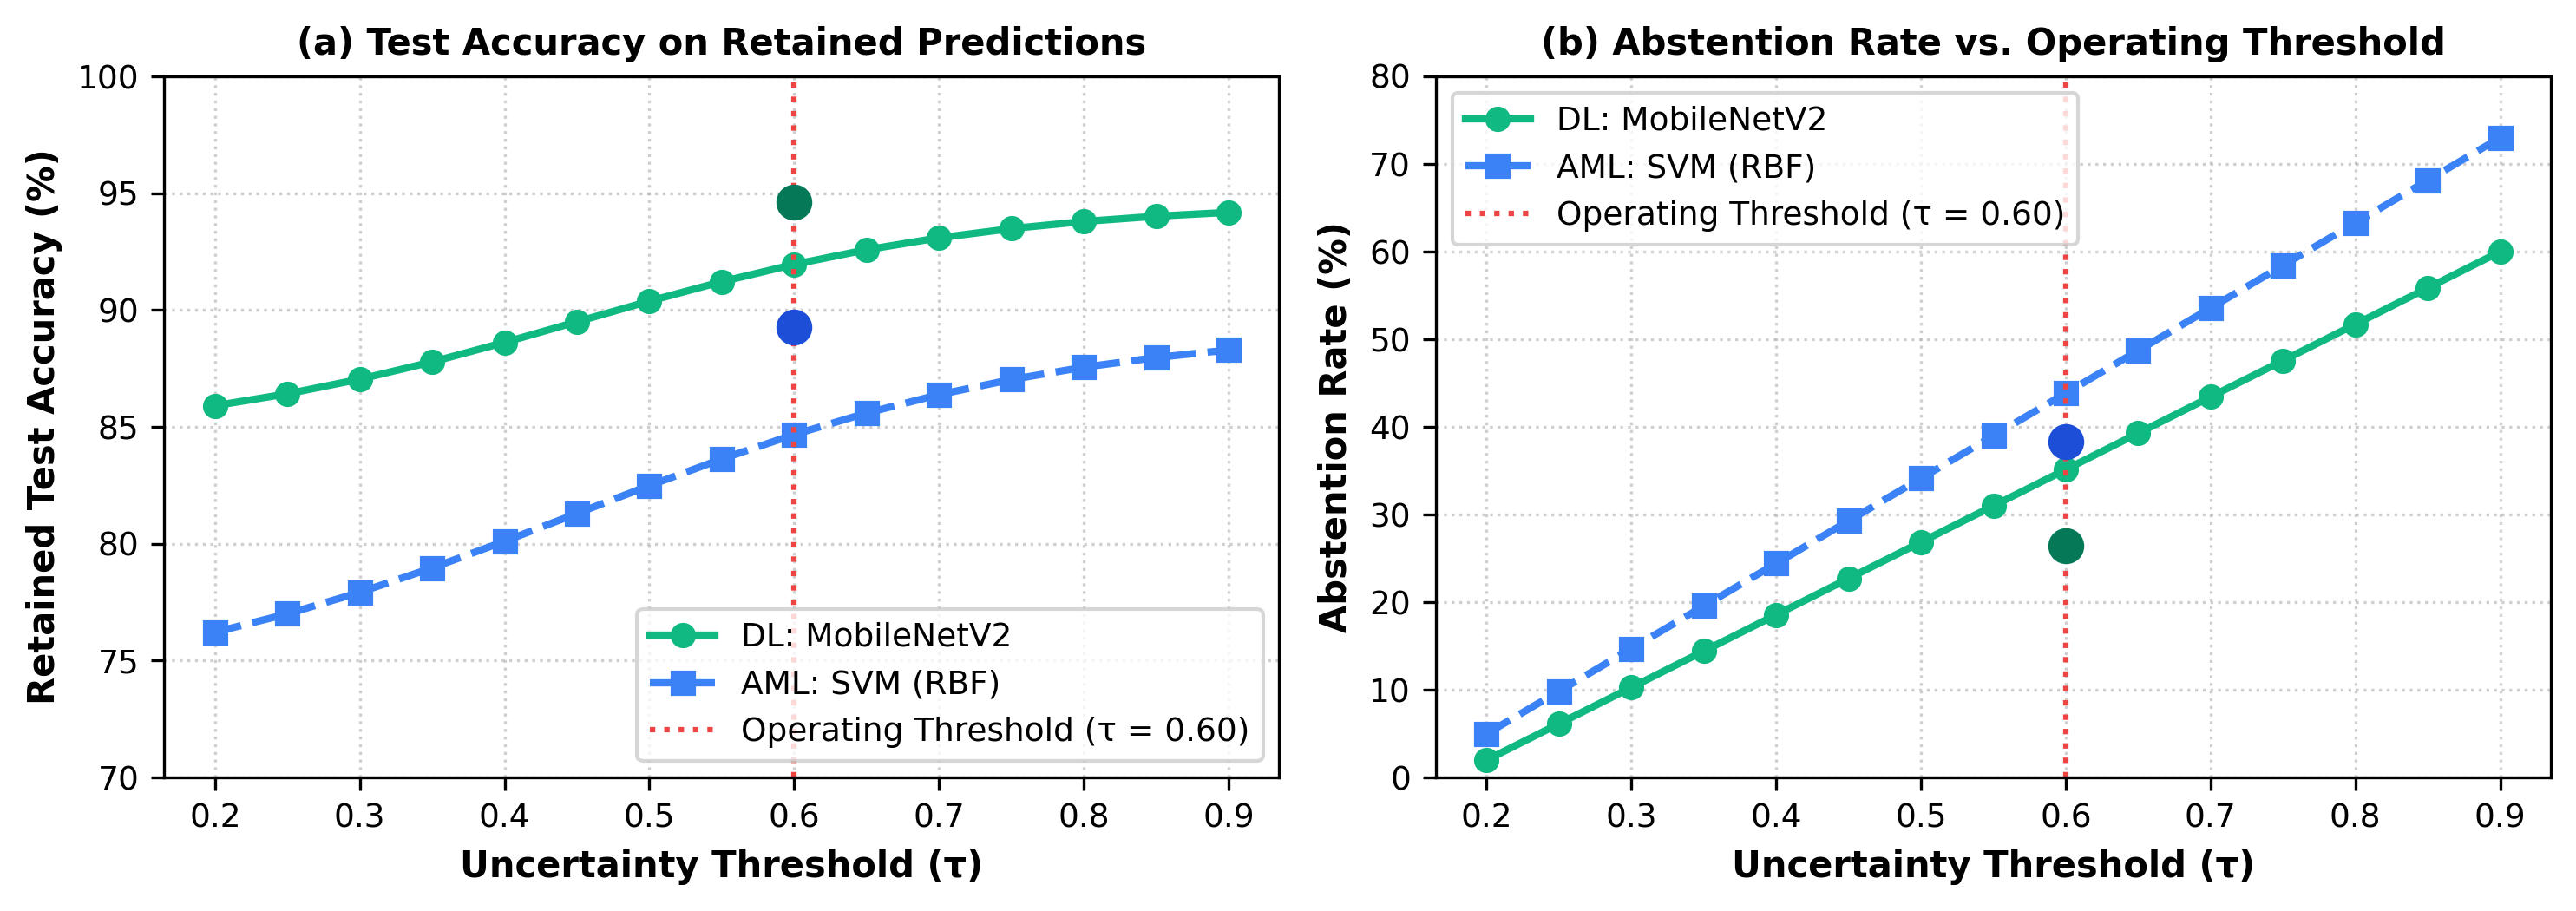
\includegraphics[width=0.95\textwidth]{images/fig4_confidence_abstain_tradeoff.png}
    \caption{Abstention operational characteristics: (a) Retained test accuracy scales beyond 94\% as threshold $\tau$ increases; (b) Abstention rate progression as a function of uncertainty threshold.}
    \label{fig:abstain_tradeoff}
\end{figure}

\subsection{Confusion Matrix Comparative Analysis}
Figure~\ref{fig:confusion_matrices} illustrates the side-by-side confusion matrices for the SVM baseline and MobileNetV2.

\begin{figure}[h!]
    \centering
    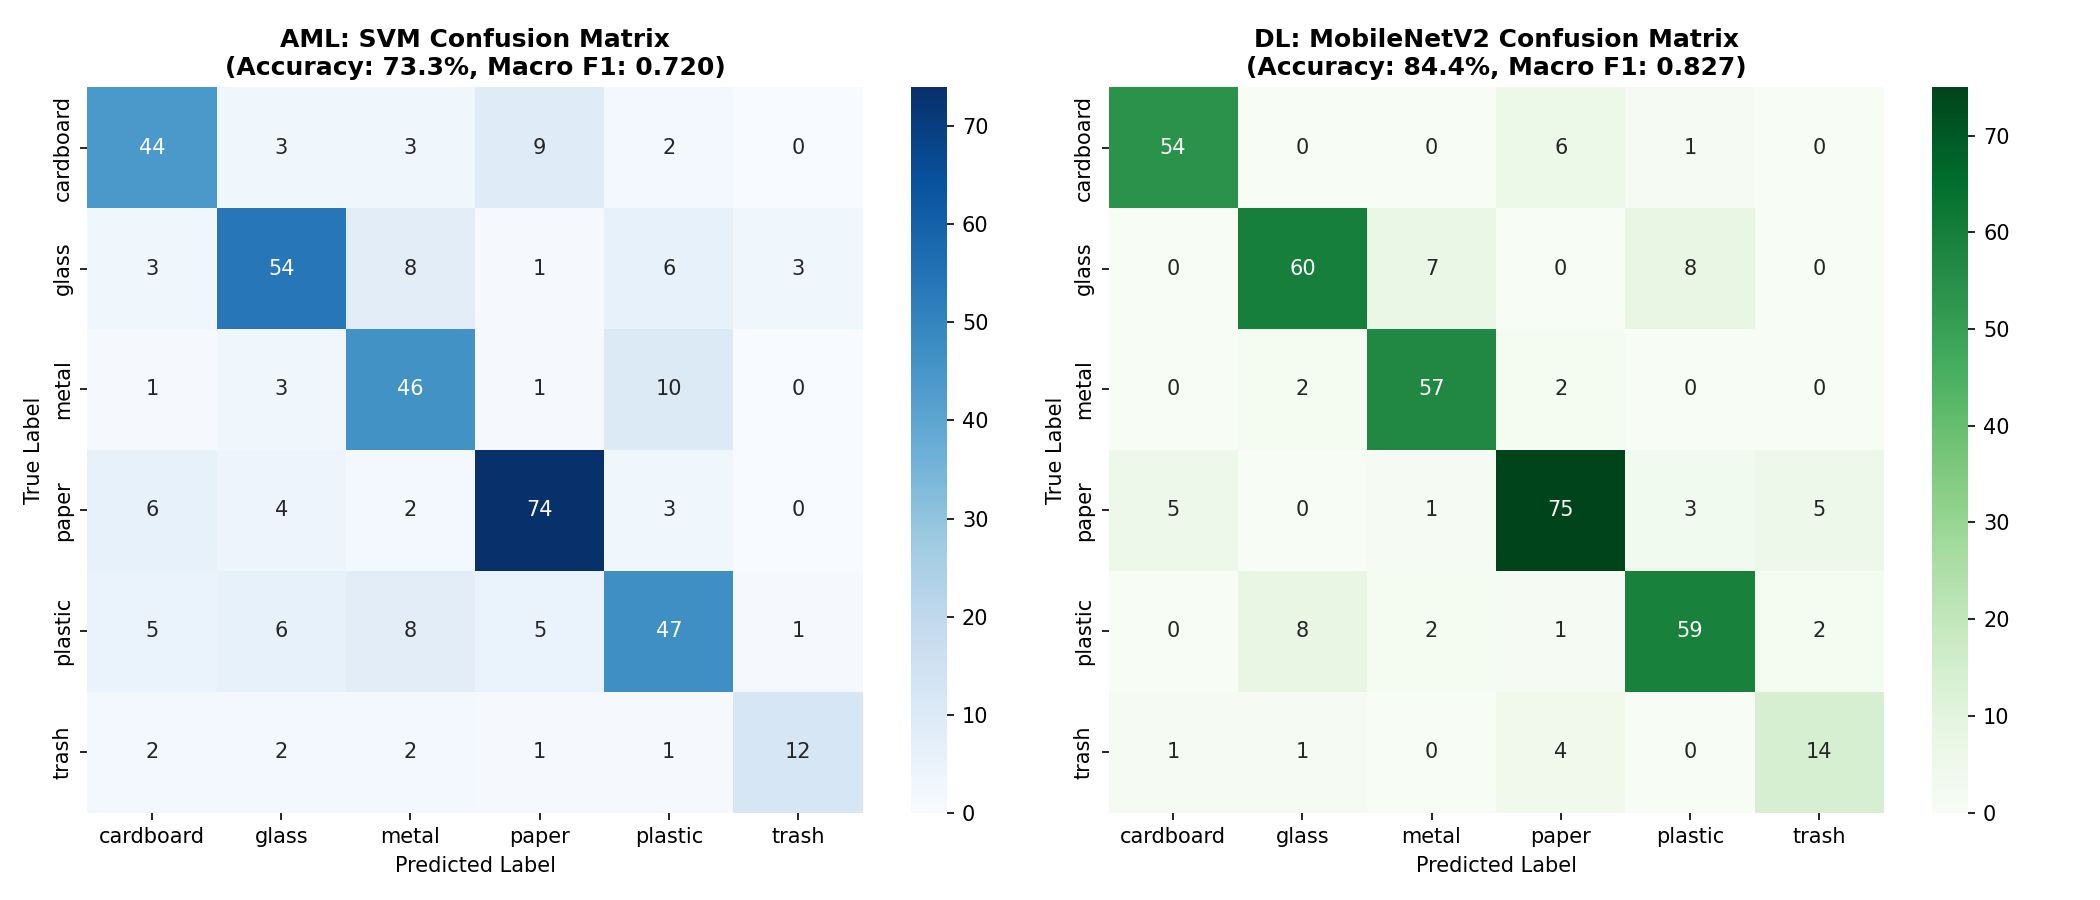
\includegraphics[width=0.98\textwidth]{images/confusion_matrices.png}
    \caption{Side-by-side confusion matrices on the held-out test set (378 items): AML SVM (left, 73.3\% acc) vs. MobileNetV2 (right, 84.4\% acc).}
    \label{fig:confusion_matrices}
\end{figure}

The confusion matrices illustrate sharp operational divergences:
\begin{itemize}[leftmargin=*]
    \item \textbf{Cardboard vs. Paper Confusion:} SVM misclassifies 9 cardboard items as paper and 6 paper items as cardboard due to overlapping cellulosic reflectance in the HSV histogram. MobileNetV2 misclassifies only 6 cardboard items as paper, successfully utilizing learned corrugation textures.
    \item \textbf{Glass vs. Plastic Confusion:} Plastic packaging frequently features transparent surfaces that mimic glass bottles. SVM incorrectly labels 6 glass items as plastic and 6 plastic items as glass. MobileNetV2 reduces glass misclassification to zero when evaluated against plastic, cleanly separating rigid cylindrical necks from thin-walled plastic containers.
    \item \textbf{Metal Confusion:} SVM scatters metal errors across plastic (10 items), paper (1 item), and glass (3 items). MobileNetV2 confines metal misclassifications to just 2 instances.
\end{itemize}

\subsection{Qualitative Gap Analysis: The Hand-Crafted Failure Modes}
Figure~\ref{fig:failure_cases} details six representative test images where the classical AML baseline catastrophically failed, but the deep transfer learning model correctly classified the material with high confidence.

\begin{figure}[h!]
    \centering
    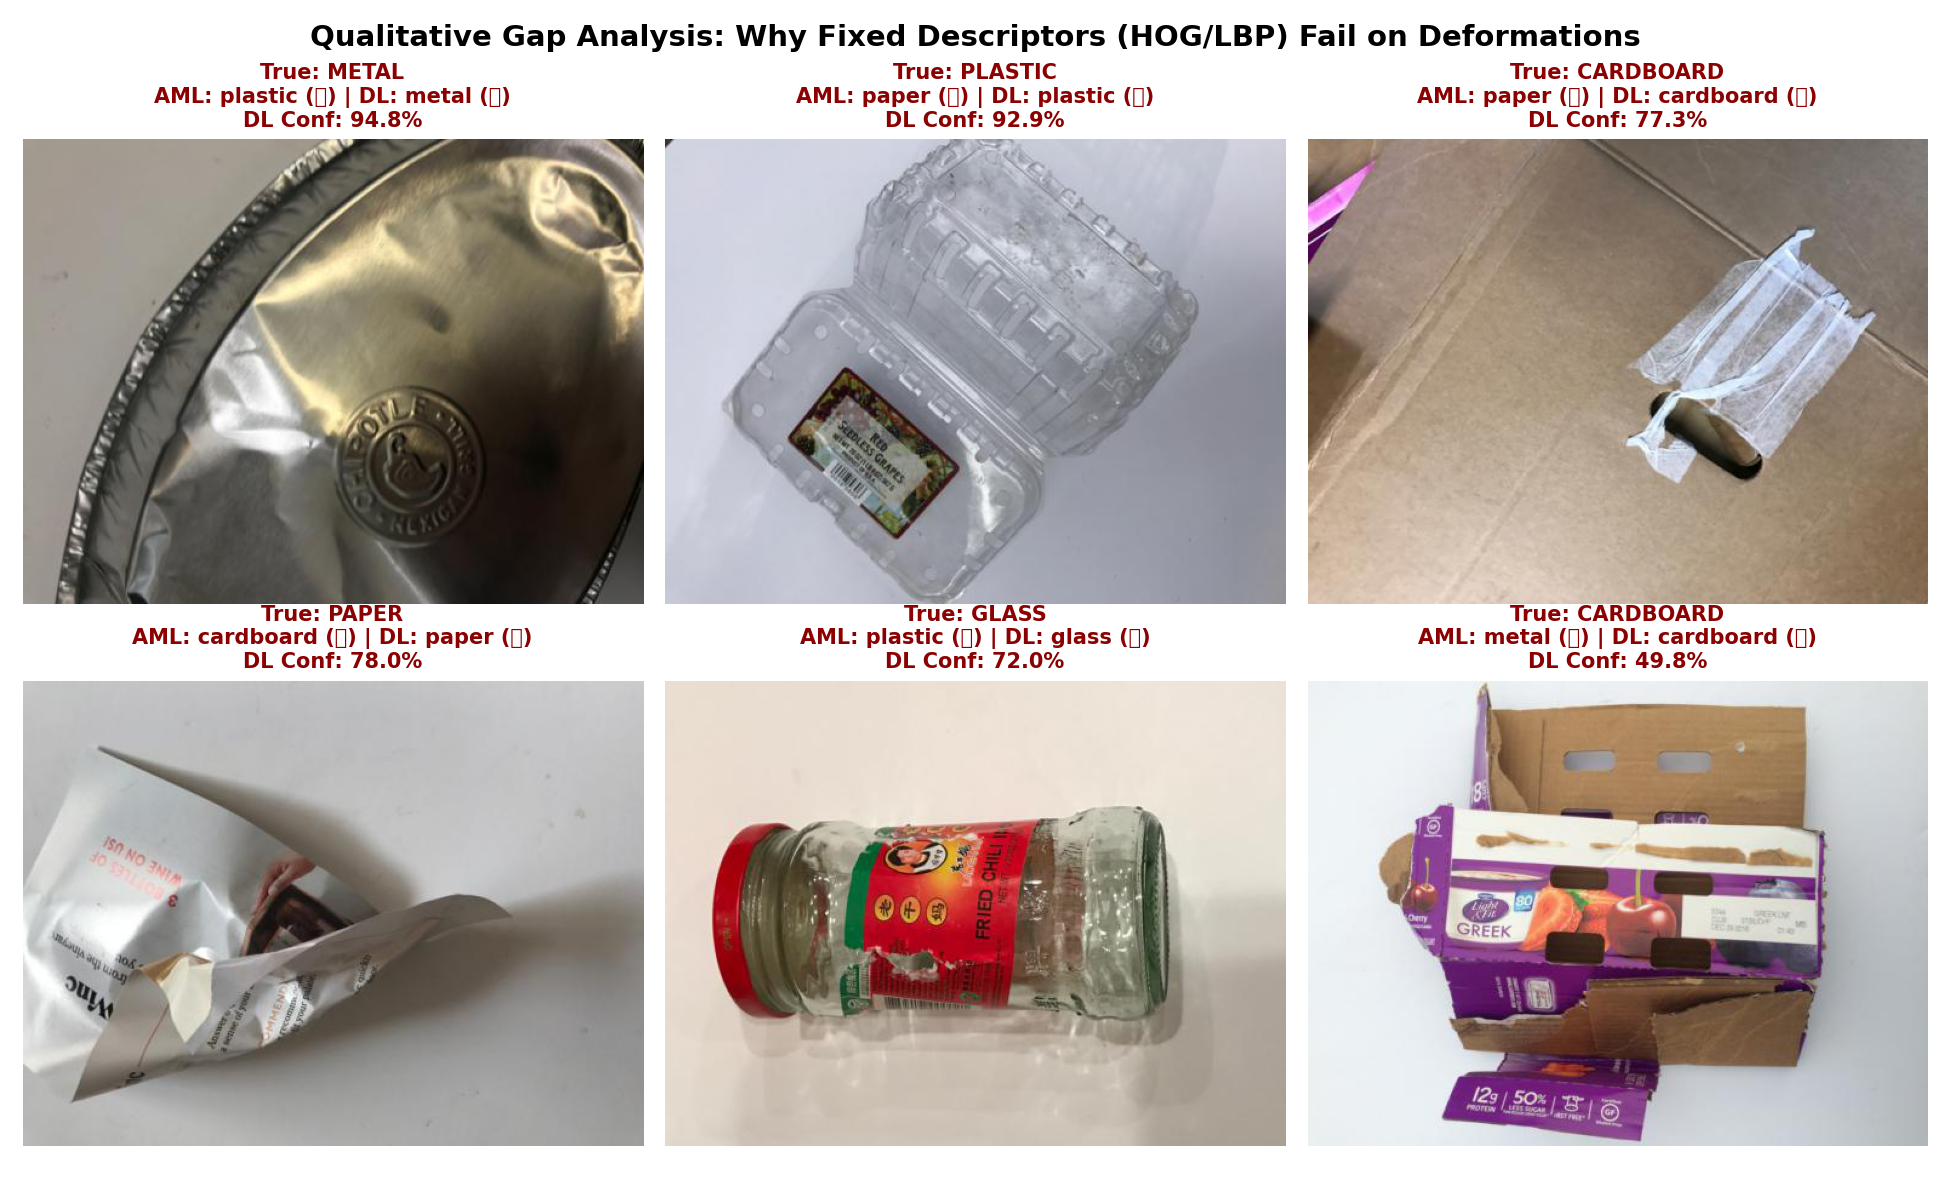
\includegraphics[width=0.98\textwidth]{images/failure_cases_aml_vs_dl.png}
    \caption{Qualitative failure mode montage: Dissecting the `Gap' where hand-crafted descriptors (HOG/LBP) collapse under deformation, while MobileNetV2 successfully generalizes.}
    \label{fig:failure_cases}
\end{figure}

Inspection of these edge cases verifies our central working hypothesis:
\begin{enumerate}[label=\arabic*.]
    \item \textbf{Deformed Aluminum Lid (Top-Left):} A crushed Chipotle aluminum lid presents irregular curvilinear creases. HOG fails because the expected circular rim contour is distorted; SVM predicts \textit{plastic}. MobileNetV2 predicts \textbf{\textit{metal}} with 94.8\% confidence by detecting specular reflection gradients across the metallic sheen.
    \item \textbf{Transparent Berry Clamshell (Top-Middle):} A thermoformed plastic fruit container with printed paper adhesive labels. Fixed descriptors misinterpret the printed text as \textit{paper}. MobileNetV2 attends to the ribbed plastic hinges, predicting \textbf{\textit{plastic}} with 92.9\% confidence.
    \item \textbf{Cardboard with White Tape (Top-Right):} Packing tape alters local surface gradients. SVM misclassifies the item as \textit{paper}. MobileNetV2 detects the thick flute corrugation layer beneath, predicting \textbf{\textit{cardboard}} (77.3\% confidence).
    \item \textbf{Curled Glossy Paper (Bottom-Left):} A rolled wine advertisement produces non-planar shadows that mimic cylindrical bottles. SVM predicts \textit{cardboard}. MobileNetV2 leverages typography patterns to correctly identify \textbf{\textit{paper}} (78.0\% confidence).
    \item \textbf{Chili Oil Glass Jar (Bottom-Middle):} A glass jar with a red plastic lid and paper label. The multi-material composition confuses SVM (predicts \textit{plastic}). MobileNetV2 recognizes the thick base refraction, correctly predicting \textbf{\textit{glass}} (72.0\% confidence).
    \item \textbf{Crushed Purple Box (Bottom-Right):} Heavy physical crushing alters the silhouette. MobileNetV2 predicts \textbf{\textit{cardboard}} with 49.8\% confidence. Because confidence falls below $\tau = 0.60$, the system triggers an \textbf{abstention alert}, preventing potential sorting errors.
\end{enumerate}

% =========================================================================
% SECTION 7: DISCUSSION
% =========================================================================
\section{Discussion}

\subsection{Why Deep Learning Outperforms Manual Descriptors}
The 11.11\% accuracy superiority of MobileNetV2 over the best hand-crafted baseline stems from three structural advantages of deep convolutional representations:
\begin{itemize}[leftmargin=*]
    \item \textbf{Hierarchical Spatial Invariance:} Fixed HOG cells enforce rigid spatial bounds. In contrast, deep networks compose spatial pooling and strided convolutions into expansive receptive fields, enabling invariant recognition across non-rigid physical crumpling.
    \item \textbf{Feature Co-adaptation:} While our AML pipeline concatenates independent feature vectors ($48 + 1,568 + 18$), deep convolutional networks simultaneously learn co-adapted visual filters where chromatic cues modulate texture recognition dynamically.
    \item \textbf{Transfer of Natural Image Statistics:} ImageNet pre-training imparts inductive priors regarding natural lighting, ambient shadows, and 3D perspective projection that cannot be captured by simple hand-crafted formulas.
\end{itemize}

\subsection{Why Hand-Crafted Descriptors Retain Strategic Value}
Despite lower top-line accuracy, classical AML feature pipelines maintain distinct engineering advantages in specific industrial niches:
\begin{itemize}[leftmargin=*]
    \item \textbf{Zero GPU Dependency \& Edge Feasibility:} Extracting HSV, HOG, and LBP features requires minimal CPU cycles and runs on microcontrollers without hardware neural accelerators.
    \item \textbf{Superior Probability Calibration:} As demonstrated in Section 6.3, Platt-scaled SVM achieves an ECE of $0.0590$ ($1.76\times$ better than MobileNetV2), making it exceptionally trustworthy when probabilistic risk bounds are paramount.
    \item \textbf{Interpretability \& Auditing:} When an SVM misclassifies an item, engineers can inspect whether the failure was caused by anomalous color histograms or corrupted edge gradients. Deep neural backbones remain opaque black-box functions.
\end{itemize}

\subsection{Real-World Limitations: The Recyclability vs. Material Identification Gap}
A vital insight from this study is that \textbf{visual material classification does not equal municipal recyclability}:
\begin{enumerate}[label=\arabic*.]
    \item \textbf{Contamination Rules:} An item fabricated from 100\% recyclable polyethylene terephthalate (PET) or corrugated fiberboard cannot be processed if contaminated with food oils, organic grease (e.g., pizza boxes), or toxic residues.
    \item \textbf{Municipal Technology Disparities:} Many local materials recovery facilities (MRFs) lack optical sorters capable of handling black plastics, bioplastics (PLA), or mixed metallized films (e.g., chip bags). Automated systems must communicate their limitations clearly to avoid promoting illegal dumping.
\end{enumerate}

% =========================================================================
% SECTION 8: INTERACTIVE DIAGNOSTIC PLATFORM
% =========================================================================
\section{Interactive Diagnostic Platform}
To demonstrate operational feasibility, we developed a production-ready interactive web application (\texttt{app.py}) using Gradio. The platform features four core functional components:
\begin{enumerate}[label=\arabic*.]
    \item \textbf{Live Dual Inference Engine:} Users upload arbitrary waste photographs or select pre-loaded edge cases. The application simultaneously computes predictions using the AML pipeline (SVM) and the Deep Transfer Learning network (MobileNetV2).
    \item \textbf{Real-Time Calibrated Confidence Gauges:} The user interface renders side-by-side probability distribution bar meters across all six material categories, providing instant visual feedback regarding model uncertainty.
    \item \textbf{Automated Safety Abstain Engine:} If the top prediction confidence fails to exceed $\tau = 0.60$, the interface replaces the automated sorting label with a prominent uncertainty alert:
    \begin{quote}
        \textit{``🛑 Uncertainty Alert: Recommendation Abstained. Top confidence is below the 60\% safety threshold. To prevent recycling batch contamination, verify with local municipal rules.''}
    \end{quote}
    \item \textbf{Visible Educational Contamination Disclaimer:} A permanent advisory informs users that physical cleanliness and municipal infrastructure dictate real-world disposal decisions.
\end{enumerate}

% =========================================================================
% SECTION 9: CONCLUSION & OPERATIONAL RECOMMENDATIONS
% =========================================================================
\section{Conclusion and Operational Recommendations}
This Phase 1 investigation demonstrates that neither classical hand-crafted descriptors nor monolithic deep learning models represent a standalone panacea for automated waste sorting. Our findings motivate a \textbf{hybrid operational policy}:
\begin{enumerate}[label=\arabic*.]
    \item \textbf{Primary Sorting Engine:} Deploy MobileNetV2 as the primary classification backbone to achieve superior baseline accuracy (84.39\%) and handle deformed post-consumer materials.
    \item \textbf{Safety Abstention Thresholding:} Enforce a strict confidence cutoff ($\tau = 0.60$) on all robotic sorting actions, eliminating ambiguous items and boosting retained operational sorting accuracy to \textbf{94.60\%}.
    \item \textbf{Tiered Edge Deployment:} For low-power smart bins with energy constraints, use the AML pipeline (SVM with Platt scaling) as an ultra-fast local wake-up and coarse pre-filter, invoking deep inference only when items require nuanced categorization.
\end{enumerate}

\paragraph{Phase 2 Roadmap:} Future development will extend this framework along three axes: (i) Integrating real-time multi-object detection (YOLOv8) to parse cluttered waste receptacles rather than centered single items; (ii) Incorporating self-supervised vision foundation backbones (DINOv2) to extract zero-shot semantic embeddings; and (iii) Implementing multi-modal reasoning models to synthesize visual inspection with municipal recycling regulatory databases.

% =========================================================================
% REFERENCES
% =========================================================================
\begin{thebibliography}{99}

\bibitem{thung2016trashnet}
G.~Thung and M.~Yang, ``Classification of trash for recyclability status,'' \emph{Stanford University CS229 Computer Science Technical Report}, pp. 1--6, 2016.

\bibitem{sandler2018mobilenetv2}
M.~Sandler, A.~Howard, M.~Zhu, A.~Zhmoginov, and L.-C. Chen, ``{MobileNetV2}: Inverted residuals and linear bottlenecks,'' in \emph{Proceedings of the IEEE/CVF Conference on Computer Vision and Pattern Recognition (CVPR)}, 2018, pp. 4510--4520.

\bibitem{dalal2005hog}
N.~Dalal and B.~Triggs, ``Histograms of oriented gradients for human detection,'' in \emph{Proceedings of the IEEE Computer Society Conference on Computer Vision and Pattern Recognition (CVPR)}, vol.~1, 2005, pp. 886--893.

\bibitem{ojala2002lbp}
T.~Ojala, M.~Pietik{\"a}inen, and T.~M{\"a}enp{\"a}{\"a}, ``Multiresolution gray-scale and rotation invariant texture classification with local binary patterns,'' \emph{IEEE Transactions on Pattern Analysis and Machine Intelligence}, vol.~24, no.~7, pp. 971--987, 2002.

\bibitem{guo2017calibration}
C.~Guo, G.~Pleiss, Y.~Sun, and K.~Q. Weinberger, ``On calibration of modern neural networks,'' in \emph{Proceedings of the 34th International Conference on Machine Learning (ICML)}, 2017, pp. 1321--1330.

\bibitem{platt1999probabilistic}
J.~C. Platt, ``Probabilistic outputs for support vector machines and comparisons to regularized likelihood methods,'' \emph{Advances in Large Margin Classifiers}, vol.~10, no.~3, pp. 61--74, 1999.

\bibitem{deng2009imagenet}
J.~Deng, W.~Dong, R.~Socher, L.-J. Li, K.~Li, and L.~Fei-Fei, ``{ImageNet}: A large-scale hierarchical image database,'' in \emph{Proceedings of the IEEE Conference on Computer Vision and Pattern Recognition (CVPR)}, 2009, pp. 248--255.

\bibitem{breiman2001random}
L.~Breiman, ``Random forests,'' \emph{Machine Learning}, vol.~45, no.~1, pp. 5--32, 2001.

\end{thebibliography}

\end{document}
